\documentclass{apuntes}

\usepackage{tikztools}
\usepackage{tikz-3dplot}
\usepackage{textcomp}
\usepackage{tikz-qtree}
\usepackage{changepage}
\usepackage{listings}
\usepackage{graphicx}
% subfiguras
\usetikzlibrary{arrows}

\newcommand{\theauthor}{}
\newcommand{\thetitle}{Memoria P2\\Criptografía}
\newcommand{\rightheader}{Memoria P2}
\newcommand{\leftheader}{UAM - 2015/2016}

% Si no compila y el directorio tikzgen está creado, quitar estas dos sentencias.
%\precompileImages
%\precompileTikz

\title{Criptografía}
\author{Cristina Kasner Tourné\\Jose Antonio García del Saz}
\date{Curso 2015 - 2015 C1}

% Paquetes adicionales

% --------------------

\newcommand{\cte}{\text{Cte}}

\begin{document}
\pagestyle{plain}
\maketitle
%\abstract{Porque los apuntes de Chamizo son demasiado fáciles}

\tableofcontents
\newpage
\appendix
% Contenido.
\chapter{Ejercicios}
\section{Ejercicio 1-Seguridad perfecta}

En este ejercico nos piden implementar un programa que compruebe la seguridad perfecta.

Recordamos la definición de seguridad perfecta:

\begin{defn}[Seguridad Perfecta]
	Decimos que un criptosistema tiene seguridad perfecta si cumple:
	$$P_p(x|y) = P_p(x)$$
	Esto quiere decir que el conocimiento de texto cifrado no nos da ninguna información sobre el texto plano.
\end{defn}

Para esto hemos creado un fichero \textit{probabilidad.c} en el que implemetamos las funciones que calculan esas probabilidades.

La probabilidad $P_p(x)$ la calculamos recorriendo el fichero que tiene el texto plano y llevando la cuenta de las veces que aparece la letra i. 

\lstset{language=C, breaklines=true, basicstyle=\footnotesize}
\begin{lstlisting}


	while((l=fgetc(f))!=EOF){
		prob[l-65]++;
		longText++;
	}


\end{lstlisting}


Luego dividimos ese número entre la longitus del texto.

La probabilidad $P_p(x|y)$ la calculamos de la misma forma solo que contabilizando a la vez los caracteres del mensaje en plano y el mensaje cifrado.

\begin{lstlisting}


	while((c=fgetc(cifrado))!=EOF){
		p = fgetc(plano);
		prob[p-65][c-65]++;
		cantLetra[c-65]++;
	}
	
\end{lstlisting}

Y finalmente dividimos entre el número de veces que aparece en el texto cifrado la letra correspondiente.

En la práctica podemos probar la seguridad perfecta con dos casos distintos.

\begin{itemize}
	\item claves equiprobables
	\item claves no equiprobables
\end{itemize}

Para generar las claves equiprobables utilizamos la función random de C.

Para las claves no equiprobables hemos escrito el siguiente código:


\begin{lstlisting}


	for(i=0; i<2;i++){
		if((clave>m/2)==0){
			clave = rand() % m;
		}else break;
	}
	
	
\end{lstlisting}



De esta forma es mucho más probable que mi clave sea una clave menor que m/2 que mayor. 

Además obligamos a que la b también pertenezca a las unidades de m.

Los resultados obtenidos tras probar el código son:

\begin{center}
	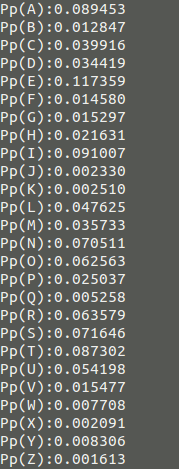
\includegraphics[width=90pt]{ProbabilidadesSimp.png}
\end{center}


\newpage
\textbf{Claves equiprobables}

\begin{center}
	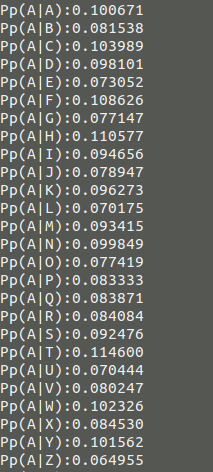
\includegraphics[width=100pt]{ProbA.png}
	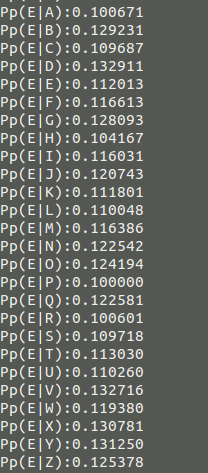
\includegraphics[width=98pt]{ProbE.png}
	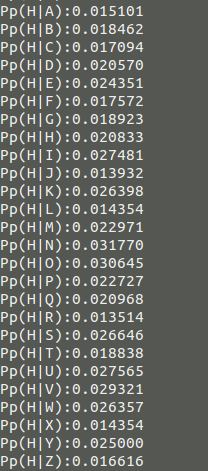
\includegraphics[width=98pt]{ProbH.png}
\end{center}

En estos ejemplos podemos ver que las probabilidades condicionadas son muy parecidas y todas tienen un valor muy cercano al de la probabilidad de la letra.

Una de las razones por las que el resultado no es exacto es que la función rand() de C no da resultados exactamente equiprobables.

\textbf{Claves no equiprobables}

\begin{center}
	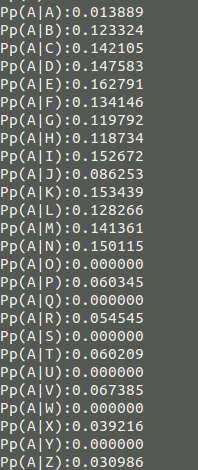
\includegraphics[width=102pt]{ProbANE.png}
	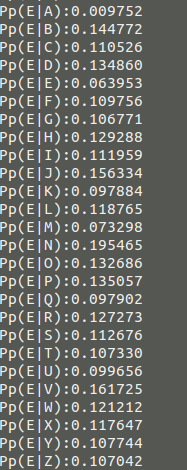
\includegraphics[width=96pt]{ProbENE.png}
	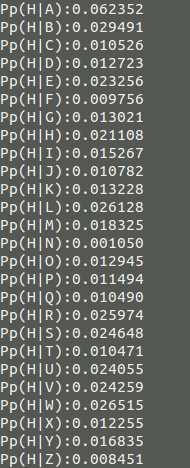
\includegraphics[width=98pt]{ProbHNE.png}
\end{center}

Vemos como estos resultados se distan mucho más que cuando utilizabamos claves probables.


\section{Ejercicio 2-Implementación del DES}

Para implementar el DES hemos creado un fichero que se llama \textit{funcionesDES.c} en el que están todas las funciones necesarias para el método.

Como sabemos el DES funciona a través de permutaciones y sustituciones(cajas-S), por esto no es ninguna sorpresa que el grueso de las funciones de \textit{funcionesDES.c} sean permutaciones y sustituciones.

Vamos a explicar ambas.

\begin{itemize}
	\item Permutaciones
	
	La idea de las funciones de permutación es la siguiente:
	
	Guardo el número que leo en la matriz de permutación, que es la posición del bit que va a ir en esa posición.
	
	Miro si ese bit es un 0 (positions[bit\%8] tiene un 1 en el bit que estoy mirando).
	
	Si es un 0 no hago nada ya que he inicializado permutation a 0.
	
	Si no es un cero meto en desired bit un 1 en la posicion apropiada y hago un 
	XOR con el byte que ya hubiera en permutation, de forma que solo cambio el bit deseado.
	
	Adjuntamos el código de una de las funciones de permutación para que se entienda mejor.
	
	\begin{lstlisting}
	
	int bit, newpos;
	unsigned char desiredbit;
	for (bit = 0; bit < 56; bit++) {
	
		newpos = ((int)PC1[bit])-1;
		desiredbit = input[newpos/8] & Positions[newpos%8]; 
		if (desiredbit != 0) {
			desiredbit = Positions[bit%8];
			permutation[bit/8] = desiredbit ^ permutation[bit/8];
		}
	}
	
	\end{lstlisting}
	
	\item Sustituciones $\rightarrow$ Cajas-S
	
	En esta función básicamente vamos rotando los bits para obtener la fila y la columna y obtenemos el resultado de las cajas-S de la siguiente forma:
	
	\begin{lstlisting}
	
	if((caja%2)==0){
		aux =S_BOXES[caja][posrow][poscolaux] <<4;
	}else{
		output[caja/2] = S_BOXES[caja][posrow][poscolaux];
		output[caja/2] =  output[caja/2] ^ aux;
		aux = 0;
	}
	
	\end{lstlisting}
	
	Esto es porque nuestra función devuelve una cadena de caracteres, cada caracter son 8 bits pero las cajas-S devuelven 4 bits por lo que vamos guardando los resultados de dos en dos.
	
\end{itemize}

Para encriptar se tiene que ejecutar el código tal y como indica el enunciado.

La clave para desencriptar aparece por terminar cuando encriptas.

Vamos a ver un ejemplo:

\begin{center}
		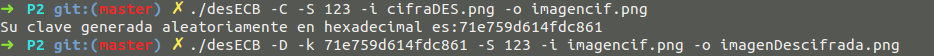
\includegraphics[width=400pt]{EjecutaDES.png}
\end{center}



\section{Ejercicio X-Estudiar la linealidad de las cajas-S del AES}

Recordamos que una función lineal es aquella función $f$ que cumple que :
$$f(a + b) = f(a) + f(b)$$

Es sencillo comprobar que las cajas-S no cumplen esto. Hemos creado un sencillo programa al que le pasas dos bytes $a$ , $b$ y aplicamos la caja-S a cada uno de ellos y sumamos los resultados.

A su vez el programa suma $a + b$ y aplica la caja-S a dicha suma y vemos que los resultados son distintos.

La no linealidad de las cajas-S del AES es muy importante ya que las hacen resistentes al criptoanálisis lineal.

\section{Ejercicio X - SAC y BIC para las cajas-S del DES}

Primero vamos a explicar qué es cada uno de estos principios.

\begin{itemize}
	
	\item \textbf{SAC} (Strict avalanch criterion)
	
	Este principio dice que la probabilidad de cambio debe estar equidistribuida.
	
	Esto es, que si cambio un bit de entrada, la probabilidad de que un bit de salida sea 0 o 1 es la misma.
	$$\forall i,j\text{  }P(c_i=1|\overline{b_j})= P(c_i=0|\overline{b_j}) = \frac{1}{2}$$
	Siendo $\overline{b_j}$ que he cambiado el bit $b_j$
	
	\item \textbf{BIC} (bit independence criterion)
	
	Busca que no haya dependencia entre los bits de salida (si cambia $c_3$, no condiciona a que cambie o no $c_2$) 
	$$\forall i,j,k \text{  } P(c_ic_j|\overline{b_k}) = P(c_i|\overline{b_k})\cdot P(c_j|\overline{b_k})$$
	
	Para comprobar esto hemos hecho un programa que cuenta la probabilidad de 0 y 1 de cada bit de salida de las cajas-S para las 64 posibles entradas.
	
	Vemos que las probabilididades son todas $0.5$, por lo que \textbf{se cumple el criterio SAC}.
	
	Para BIC no comprobamos que $ P(c_ic_j|\overline{b_k}) = P(c_i|\overline{b_k})\cdot P(c_j|\overline{b_k})$, sino que
	$$ P(c_ic_jc_kc_l|\overline{b_k}) = P(c_i|\overline{b_k})\cdot P(c_j|\overline{b_k})\cdot P(c_k|\overline{b_k})\cdot P(c_l|\overline{b_k})$$

	Para esto calculamos $P(c_ic_jc_kc_l|\overline{b_k})$, que nos sale $ 0.0625$.
	
	Las probabilidades $P(c_i|\overline{b_k})$ ya las habiamos calculado para el SAC y habíamos vist que son todas iguales, por lo que si hacemos $(0.5)^4$ vemos que nos da $0.0625$.
	
	Por lo que queda comprobado que también cumple BIC.
	
	Adjuntamos dos pantallazos de la salida. En la imagen de la izquierda vemos las probabilidades de cada bit de salida de ser 0 o 1.
	
	En la imagen de la derecha vemos las probabilidades $P(c_ic_jc_kc_l|\overline{b_j})$
	
	\begin{center}
		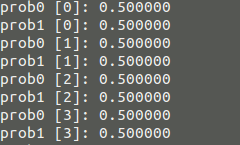
\includegraphics[width=180pt]{SACBICDES1.png}
		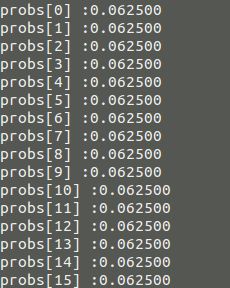
\includegraphics[width=150pt]{SACBICDES2.png}
	\end{center}
\end{itemize} 

\printindex
\end{document}